\documentclass[12pt]{article}

\usepackage[ngerman]{babel}
\usepackage[utf8]{inputenc}
\usepackage{amssymb}
\usepackage{amsmath}
\usepackage{gensymb}
\usepackage{color}
\usepackage{graphicx}
\usepackage{wrapfig}
\usepackage{svg}
\usepackage{listings}
\usepackage[hidelinks]{hyperref}

\begin{document}

\begin{titlepage}
	\centering
	
\includegraphics[width=0.2\textwidth]{Bilder/hszg}\par
	\vspace{1cm}
	{\LARGE Hochschule Zittau/Görlitz \par}
	\vspace{1cm}
	{\Large Mobile Anwendungen\par}
	\vspace{1.5cm}
	{\huge\bfseries FacilityManager \par}
	\vspace{0.75cm}
	{\LARGE Umsetzung als hybride Ionic-App\par}
	\vspace{2cm}
	{\Large Team 1 - Backend\par}
	\vspace{0.75cm}
	{\Large Niklas Merkelt\\Uta Lemke\par}
	\vfill
	{\large 07. Februar 2020\par}
\end{titlepage}

\tableofcontents
\newpage

\begin{abstract}
Im Folgenden geht es um die Implementierung einer Hausmeister-App, von uns FacilityManager getauft, mit der Schadensmeldungen verfasst und abgeschickt, Objektkontrollen anhand von Checklisten durchgeführt und dokumentiert und Informationen über Objekte abgerufen werden können.
\paragraph{Fachlicher Aspekt}
Zu dieser App existierte anfangs bereits ein Prototyp, neu ist allerdings die Zusammenführung aller Funktionen in einer Anwendung und die Möglichkeit, Objektkontrollen mithilfe der App durchzuführen. Außerdem war vorgegeben, dass die neue Auflage der Hausmeister-App auch offline funktioniert, was durch eine interne Wrapper-Datenbank für die per RESTful-Webservice erreichbare bereits vorhandene Datenbank realisiert werden sollte. Mehr dazu in Abschnitt \ref{sec:aufg}.
\paragraph{Technologie}
Damit die App auf möglichst vielen Plattformen läuft, haben wir uns am Anfang des Projekts für die Umsetzung mit dem Ionic-Framework entschieden. Dieses ermöglichte uns ein Arbeiten auf hohem Abstraktionsniveau bei gleichzeitigem Handhaben der Implementierung auf Android, iOS, als Web-App, Electron-App, etc.
\paragraph{Organisation}
Zu Beginn wurde das Projekt auf drei Arbeitsteams aufgeteilt, ein Team für das Backend, ein Team für den Schadensmeldungsteil der GUI und ein Team für den Objektkontrollenteil der GUI. Hier soll es um den Beitrag des ersten dieser Teams gehen.
\end{abstract}

\section{Aufgabenstellung}\label{sec:aufg} 
Unser Team hatte den Auftrag, sich die folgenden Teile der App zu kümmern:
\paragraph{Das Backend} Eine Datenbankinfrastruktur, die den Zwischensicht zwischen Webservice und der restlichen App bildet. Hierbei soll sichergestellt werden, dass regelmäßig die aktuellen Daten über Objekte, Mitarbeiter, Schadensmeldungen und Vorlagen für Objektkontrollen heruntergeladen werden und der App dann im Offline-Betrieb zur Verfügung stehen. Außerdem soll eine Schnittstelle bereitgestellt werden, die das Abfragen der lokal gespeicherten Daten erlaubt, ohne dabei direkt auf die per Webservice bereitgestellten Datenbanken zuzugreifen. Auch weitere interne App-Daten sollen nach Bedarf in der internen Datenbank gespeichert werden können. Die entsprechende Datenanalyse war dann Aufgabe der anderen beiden Teams.
\paragraph{Die Webserviceschnittstellen} Neben dem Bereitstellen von Daten aus den entsprechenden Webservice-Endpunkten, war es auch Aufgabe, eine einheitliche Schnittstelle zur Sendung von Daten an den Webservice einzurichten. Bei Internetverbindung sollen ausstehende Schadensmeldungen und vollendete Objektkontrollen an die entsprechenden Endpunkte des Webservices geschickt werden, ansonsten werden auch diese in der internen Datenbankstruktur gespeichert.
\paragraph{Die Authentisierung} Hier geht es darum, dass der Mitarbeiter, welcher eine Schadensmeldung oder abgeschlossene Objektkontrolle versenden möchte, authentifiziert werden kann. Dafür sollten wir eine Art Login-System mitsamt grafischer Oberfläche bauen, in welchem bei Erstkonfiguration der App der zuständige Administrator den Mitarbeiter und optionale Berechtigungen des Selbigen einstellen kann. Zu diesen Berechtigungen zählt bis jetzt nur die Objektkontrolle, welche nur einige der Angestellten durchführen können sollen. Dieser Bereich soll außerdem passwortgeschützt sein, wobei es dabei weniger um hohe Sicherheitsanforderungen geht, als vielmehr um Prozessoptimierung, der Angestellte selbst soll sich um keine Konfiguration mehr kümmern müssen und können. Als Ergebnis dieser Einstellungen wird angegebene Name des Mitarbeiters bei jedem gesendeten Bericht automatisch eingetragen und die Funktion der Objektkontrolle wird entweder an- oder ausgeschaltet, was auch zu einer Anpassung der Benutzeroberfläche führen soll.
\paragraph{Der Anwendungsrahmen} Zusätzlich wurde unserem Team die Verantwortung übertragen, die Projektstruktur vorzugeben und sich um die Einrichtung der Versionsverwaltung zu kümmern.

\newpage
\section{Lokale Datenbankinfrastruktur}
Die lokale Datenbankinfrastruktur, dient dazu die Daten auf dem Gerät für den Fall vorzuhalten, dass keine Verbindung zum Internet, beziehungsweise Webservice, möglich ist, um die App auch in diesem Fall nutzen zu können.

\paragraph{}Da die Applikation auf verschiedenen Plattformen lauffähig sein soll, muss die entsprechende Speichertechnologie auf die Plattformen abgestimmt sein, auf denen die App läuft. Dafür wird das Modul Ionic Storage vom Ionic-Framework bereitgestellt. Mit Ionic Storage können verschiedene Speichertechnologien, je nach Verfügbarkeit auf der jeweiligen Plattform, verwendet werden. So wird  in folgender Reihenfolge versucht, die Datenbanksysteme zu benutzen: SQLite, IndexedDB, WebSQL und Localstorage. Zum Beispiel wird in den Applikationen auf Android und iOS das Datenbanksystem SQLite verwendet. Wenn die Anwendung im Webbrowser läuft, dann wird in modernen Browsern IndexedDB verwendet, sollte das nicht verfügbar sein, WebSQL oder Localstorage. 

\paragraph{}Die Daten werden auf dem Gerät in den folgenden sechs Key-Value-Daten"-banken gespeichert: \texttt{\_checklists} (Objektkontrollen), \texttt{\_damages} (Schadensmeldungen), \texttt{\_defaultChecklists} (Vorlagen für Objektkontrollen), \texttt{\_employees} (Mitarbeiter), \texttt{\_properties} (Objekte) und \texttt{\_settings} (Einstellungen der App).

\paragraph{}Die Datenbanken \texttt{\_checklists} und \texttt{\_damages} speichern gesendete und zu sendende Objektkontrollen und Schadensmeldungen. Dafür gibt es in jeder der Datenbanken zwei JSON-Arrays, um gesendete und zu sendende Daten zu speichern. Über die Speicherung der Daten in zwei JSON-Arrays muss für diese Einträge keine ID generiert, beziehungsweise erfunden, werden. Dies vereinfacht die Datenhaltung, bietet aber beim Zugriff den Nachteil, immer nur das komplette Array abfragen zu können. Diese Datenbanken stellen sowohl sicher, dass die Objektkontrollen und Schadensmeldungen auch im Offline-Betrieb erfasst und später gesendet werden können, als auch, dass die bereits gesendeten Objektkontrollen und Schadensmeldungen in der App angezeigt werden können.

\paragraph{}Die Datenbanken \texttt{\_defaultChecklists}, \texttt{\_employees} und \texttt{\_properties} speichern Vorlagen für Objektkontrollen, Mitarbeiter und Objekte. Diese Datensätze werden an Hand der jeweiligen ID in die entsprechende Datenbank gespeichert. Dabei werden nur die relevanten Daten aus den jeweiligen JSON-Objekten, welche vom Webservice abgerufen wurden, in die Datenbank übernommen. Diese Datenbanken dienen lediglich zur Vorhaltung für den Offline-Betrieb.

\paragraph{}Die Datenbank \texttt{\_settings} speichert die Einstellungen der App. Sie wird unter anderem dafür verwendet, den aktuellen Mitarbeiter zu speichern und ob Objektkontrollen auf diesem Gerät zugelassen sind. Über den von uns bereitgestellten \texttt{SettingsService} können von allen App-Komponenten weitere Schlüssel-Wert-Paare gespeichert und abgerufen werden.

\section{Kommunikation mit dem Webservice}
Für die Datenflusskontrolle zwischen App und Datenbank des Kunden wurde uns ein Webservice mit insgesamt fünf Endpunkten zur Verfügung gestellt. Drei davon dienen der Abfrage von Daten. Dabei handelt es sich um Informationen zu Objekten, den Mitarbeitern und Vorlagen für die Objektkontrollen. Mit den anderen beiden Endpunkten werden neue Schadensmeldungen und abgeschlossene Objektkontrollen verschickt.

\paragraph{}Um die verschiedenen Webserviceendpunkte dem Rest der App zur Verfügung zu stellen, wurden als Interface Angular-Services kreiert. Diese werden dann in jeder Klasse, welche die Funktionalität nutzen möchte, injiziert, sodass es von jedem Service nur eine, global verfügbare Instanz gibt.\\ \ \\
Hierbei gibt es die folgenden Services:
\paragraph{Der DamageService}
Mit diesem Service können neue Schadensmeldungen verschickt werden. Sollte zum Zeitpunkt des Sendeversuchs keine Internetverbindung bestehen, werden die ausstehenden Schadensmeldungen in ein JSON-Array zwischengespeichert, welches auch in der Datenbank unter dem Schlüssel \texttt{TO\_SEND} abgespeichert wird, damit diese ausstehenden Schadensmeldungen im Falle einer Schließung der App nicht verlorengehen. Sobald dann wieder eine Internetverbindung besteht, kann die Methode \texttt{sendPending""Damages} aufgerufen werden, mit der die Schadensmeldungen an den Webserviceendpunkt geschickt und dann als gesendet markiert werden.
\paragraph{Der EmployeeService} Dieser Service stellt Informationen zu einem gegebenen Mitarbeiter sowie eine Liste aller Mitarbeiter zur Verfügung. Außerdem können Einstellungen wie der aktuell in der App eingetragene Mitarbeiter und die Berechtigungen des Selbigen abgefragt werden.
\paragraph{Der ObjectChecklistService} Mit diesem Service können sowohl Vorlagen für Objektkontrollen abgerufen als auch fertiggestellte Objektkontrollen abgeschickt werden. Analog zum \texttt{DamageService} werden auch hier bei nicht vorhandener Internetverbindung die zu sendenden Objektkontrollen in ein JSON-Array geschrieben, welches dann, sobald die App wieder Onlinezugriff hat, abgearbeitet wird, um die ausstehenden Kontrollen zu verschicken.
\paragraph{Der PropertyService} Der Name dieses Services hat zuerst zu Verwirrung geführt, da wir im Rahmen dieses Projekts meist von ``Objekten'' geredet, weshalb man nun auch als Bezeichner \texttt{Object} und dementsprechend \texttt{ObjectService} erwarten würde. Allerdings ist \texttt{object} in TypeScript ein nicht verwendbares Schlüsselwort, weshalb wir uns auf den Namen \texttt{Property} geeinigt haben. Mit diesem \texttt{PropertyService} können nun einzelne Objekte mit ID abgefragt sowie Listen von Objekten nach Stadt oder eine Gesamtliste aller Objekte zurückgegeben werden. Wie auch beim \texttt{EmployeeService} kann hier ein Update der Property-Daten ausgelöst werden. Als Dummy-Objekt für den Objektexplorer gibt es zusätzlich noch die Möglichkeit der Generierung eines leeren Property-Objekts.

\section{Datensynchronisierung}
Es soll nur mit dem Webservice kommuniziert werden, wenn das Gerät auch wirklich online ist und wenn es überhaupt sinnvoll ist, die Daten zu synchronisieren. Hierzu wurde ein \texttt{NetworkListener} implementiert, was sich als schwieriger als gedacht herausstellte, dazu später mehr.\\
Zu Anfang wurde bei jeder Abfrage einer Information diese direkt vom Webservice abgefragt und in aktualisierter Form in die interne Datenbank geschrieben. Um den zusätzlichen Zeitaufwand dieser Synchronisierung zu vermeiden, wird sie nun nur noch bei Start der App, wenn die App aus einem Offline- in einen Onlinezustand kommt und bei manuellem Synchronisierungsaufruf in der Benutzeroberfläche durchgeführt. Die App arbeitet somit nach der Synchronisierung beim Start nur noch mit der internen Datenbank.

\paragraph{}
Die Verwaltung der Onlinefunktionalität der App wurde mit folgenden Komponenten umgesetzt: 
\paragraph{Der NetworkSendService} Dieser Service führt auf Anfrage von allen Services die Synchronisationsfunktionen zum Abschicken ausstehender Meldungen und Herunterladen der aktuellen Daten vom Webservice aus.
\paragraph{Der NetworkQueryService} Dieser gibt auf Anfrage den Onlinestatus der App zurück. Anfangs war diese Funktion auch Teil des \texttt{NetworkSendService}. Allerdings kam es dadurch zu Problemen mit Circular Imports, da die Services, die Daten an den Webservice verschicken, zunächst den Onlinestatus abfragen, wodurch sie den Netzwerkservice importiert haben müssen. Gleichzeitig werden aber auch die Synchronisationsfunktionen dieser Services im Netzwerkservice aufgerufen, wodurch sie auch dort importiert werden müssen. Deshalb wurden diese beiden Teile voneinander getrennt.
\paragraph{Die NetworkListenerDirective} Ursprünglich sollte der \texttt{NetworkListener} auch in den Netzwerkservice integriert werden, leider bietet Angular aber keine Möglichkeit, einen HostListener (die präferierte Weise, in TypeScript nach globalen Events zu lauschen) in einen Service einzubinden. Dafür wird eine Directive benötigt, die dann in jede der GUI-Komponenten eingebunden werden kann, sodass, egal auf welcher App-Seite der User sich befindet, das Onlineevent erkannt wird. Die nächste Schwierigkeit bei dieser Umsetzung ist, dass eine Directive nicht einfach in \texttt{app.module.ts} deklariert werden kann, damit sie von allen Komponenten genutzt werden kann. Stattdessen muss ein neues Modul, hier als \texttt{CommonModule} bezeichnet, erstellt werden, welches dann auf root-Ebene deklariert und in jedem Modul importiert werden kann. Dann erst ist es möglich, die \texttt{NetworkListenerDirective} in den \texttt{ionic-body}-Tag der entsprechenden HTML-Seite einzubinden, um den \texttt{NetworkListener} dort zu nutzen.

\section{Objektexplorer}
Der Objektexplorer dient dazu, Informationen und Kontaktdaten der Handwerker, beziehungsweise Dienstleister, von einem Objekt bereitzustellen, damit soll eine schnelle Möglichkeit für die Hausmeister geschaffen werden, die Kontaktdaten der Handwerker zu finden.

\begin{wrapfigure}{r}{6cm}
	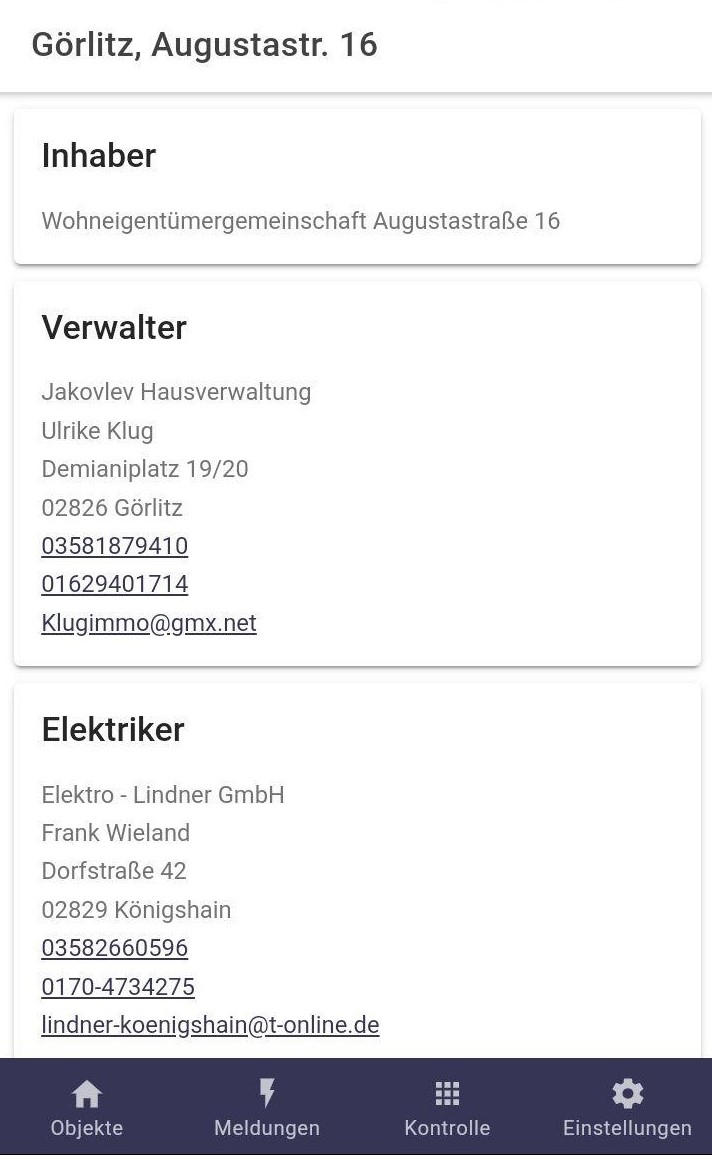
\includegraphics[width=6cm]{Bilder/object-explorer-2.jpg}
	\caption{Objektexplorer Detailansicht}
	\vspace{-0.75cm}
\end{wrapfigure}
\paragraph{}Im Tab \textit{Objekte} werden alle Objekte mit ihrer Anschrift aufgelistet und können über ein Suchfeld gefiltert werden. Wenn ein Objekt ausgewählt wird stehen die folgenden Daten über die eingetragenen Handwerker, beziehungsweise Dienstleister, zur Verfügung: Name, Anschrift, Telefonnummer, Mobilfunknummer und E-Mail-Adresse. Diese Informationen stehen nicht bei jedem Objekt zur Verfügung, da diese in der Datenbank des Webservices nicht gepflegt wurden oder nicht relevant sind. Im Moment sind folgende Handwerker, beziehungsweise Dienstleister, implementiert: Verwalter, Elektriker, Heizungsmonteur, Installateur, Schlüsseldienst, Schornsteinfeger, Brandschutz, Rohrreinigungsfirma und Fahrstuhl. Ebenfalls werden die Inhaberinformationen des Objekts auf dieser Seite angezeigt.

\paragraph{}Zuerst stand für den Abruf der Handwerker, beziehungsweise Dienstleister, nur ein Endpunkt am Webservice zur Verfügung, über welchen die Daten nur zu einem konkreten Objekt abgefragt werden konnten. Weil deshalb für jedes Objekt eine extra Anfrage an den Webservice nötig war, hat sich das Abholen der Daten für die Offline-Arbeit sehr aufgebläht. Teilweise hat sich die Abarbeitung dieser Anfragen über mehrere Minuten hingezogen.

\paragraph{}Die beste Lösung war ein neuer Webservice-Endpunkt, welcher es ermöglicht, dass die Daten aller Objekte mit einer einzigen Abfrage abgefragt werden können. Bis dieser Webservice fertiggestellt war haben wir die Daten für den Objektexplorer live abgefragt, wenn diese benötigt wurden. Währenddessen war dieser Teil der App, also nicht offlinefähig.

\section{Nutzerverwaltung}
Auf dem Gerät muss ein Nutzer ausgewählt werden, welcher dann als Absender der Objektkontrollen und Schadensmeldungen übermittelt wird. Es soll dem Nutzer aber nicht möglich sein im Namen eines anderen Mitarbeiters die App zu nutzen, außerdem soll die Nutzung der Objektkontrolle nur bestimmten Mitarbeitern vorbehalten sein.

\paragraph{}Da der Webservice im Moment keine Authentifizierung ermöglicht, wurde ein Konzept umgesetzt, bei dem die Person, welche die Geräte der Hausmeister betreut und verwaltet, Zugangsdaten für einen gesicherten Administrationsbereich bekommt und dort diese Einstellungen vornehmen kann. Dies stellt zwar wie oben genannt sicher, dass der Nutzer selbst nicht den Absender wechseln kann, heißt aber auch, dass immer der Geräteverwalter diese Einstellung ändern muss. Im gleichen Administrationsbereich legt der Verwalter ebenfalls fest, ob mit diesem Gerät Objektkontrollen durchgeführt werden dürfen. Aktuell kann das Passwort für den gesicherten Administrationsbereich nicht geändert werden und ist fest im Quellcode definiert, es wäre deshalb sinnvoll dem Verwalter zu ermöglichen, das Kennwort zu ändern.

\paragraph{}Die ideale Lösung wäre, eine Anmeldung zu implementieren, mit welcher dann der Nutzer klar authentifiziert wird. Wenn zusätzlich auch ein Merkmal am Mitarbeiter gespeichert wird, ob dieser Objektkontrollen durchführen darf, dann kann der momentane gesicherte Administrationsbereich komplett entfallen. Mit dieser Implementierung würde auch der erhöhte Arbeitsaufwand für die Betreuung der Geräte durch den Geräteadministrator entfallen. Zusätzlich bringt es den Vorteil, dass die Geräte auch von Hausmeister zu Hausmeister weitergegeben werden können, ohne vom Verwalter neu eingerichtet werden zu müssen.

\newpage
\section{Schreibanteile}

Die folgenden Abschnitte wurden von Niklas Merkelt bearbeitet:
\begin{itemize}
	\item Lokale Datenbankinfrastruktur
	\item Objektexplorer
	\item Nutzerverwaltung
\end{itemize}
Die folgenden Abschnitte wurden von Uta Lemke bearbeitet:
\begin{itemize}
	\item Aufgabenstellung
	\item Kommunikation mit dem Webservice
	\item Datensynchronisierung
\end{itemize}

\end{document}
